%%%%%%%%%%%%%%%%%%%%%%% file typeinst.tex %%%%%%%%%%%%%%%%%%%%%%%%%
%
% This is the LaTeX source for the instructions to authors using
% the LaTeX document class 'llncs.cls' for contributions to
% the Lecture Notes in Computer Sciences series.
% http://www.springer.com/lncs       Springer Heidelberg 2006/05/04
%
% It may be used as a template for your own input - copy it
% to a new file with a new name and use it as the basis
% for your article.
%
% NB: the document class 'llncs' has its own and detailed documentation, see
% ftp://ftp.springer.de/data/pubftp/pub/tex/latex/llncs/latex2e/llncsdoc.pdf
%
%%%%%%%%%%%%%%%%%%%%%%%%%%%%%%%%%%%%%%%%%%%%%%%%%%%%%%%%%%%%%%%%%%%


\documentclass[runningheads,a4paper]{llncs}

\usepackage{amssymb}
\setcounter{tocdepth}{3}
\usepackage{graphicx}
%%%%%%%%%%%%%%% New package
\usepackage{amsmath}
\usepackage{caption}
\usepackage{subfig}
%\usepackage{csvsimple}
\usepackage{multirow}
\usepackage{array}
\usepackage{booktabs}
%%%%%%%%%%%%%%%
\usepackage{url}
\usepackage{algorithm}
\usepackage{algorithmic}
\renewcommand{\algorithmicrequire}{ \textbf{Input:}} %Use Input in the format of Algorithm
\renewcommand{\algorithmicensure}{ \textbf{Output:}} %UseOutput in the format of Algorithm

% \urldef{\mailsa}\path|{soltanin, locheng, ingrid.haas, frank.holzwarth,|
% \urldef{\mailsb}\path|anna.kramer, leonie.kunz, christine.reiss, nicole.sator,|
% \urldef{\mailsc}\path|erika.siebert-cole, peter.strasser, lncs}@springer.com|
% \newcommand{\keywords}[1]{\par\addvspace\baselineskip
% \noindent\keywordname\enspace\ignorespaces#1}

\begin{document}

%\mainmatter  % start of an individual contribution

% first the title is needed
\title{Optical Flow Feature(OFF) for Human Activity Recognition in Video Game}

% a short form should be given in case it is too long for the running head
%\titlerunning{Lecture Notes in Computer Science: Authors' Instructions}

% the name(s) of the author(s) follow(s) next
%
% NB: Chinese authors should write their first names(s) in front of
% their surnames. This ensures that the names appear correctly in
% the running heads and the author index.
%
\author{Fei Yang \and Ningbo Zhu}
%\thanks{Please note that the LNCS Editorial assumes that all authors have used
%the western naming convention, with given names preceding surnames. This determines
%the structure of the names in the running heads and the author index.}%

%%
%\authorrunning{Lecture Notes in Computer Science: Authors' Instructions}
% (feature abused for this document to repeat the title also on left hand pages)

% the affiliations are given next; don't give your e-mail address
% unless you accept that it will be published
\institute{Dept. of Computing Science, University of Alberta, Canada}

%
% NB: a more complex sample for affiliations and the mapping to the
% corresponding authors can be found in the file "llncs.dem"
% (search for the string "\mainmatter" where a contribution starts).
% "llncs.dem" accompanies the document class "llncs.cls".
%

% \toctitle{Lecture Notes in Computer Science}
% \tocauthor{Authors' Instructions}
\maketitle


\begin{abstract}

	Human Activity Recognition (HAR) is one of the most popular research topics in the field of computer vision. It is widely applied in the various fields, such as on medical systems, human-computer interaction, surveillance environments, and video game. According to different recognition technologies, HAR can be divided into four main categories: HAR based on computer vision, HAR based on sensor system, HAR based on location, and HAR based on characters interaction. This paper mainly investigates the plausibility of using Optical Flow Feature for HAR in the video game field. Basically, our proposed method has three main steps: 1) Preprocessing data using optical flow, 2) Feature Extraction, 3) Classification. The Horn-Schunck optical flow method is used for the first and second step. In the classification part, histogram data analysis combined with histogram distance subtraction is used. The G3Di dataset is used for evaluation of the proposed method. Most sequences contain multiple action classes in a controlled indoor environment with a fixed camera, a typical setup for gesture-based gaming. The proposed method is shown to be promising in human activity recognition.

\end{abstract}


\section{Introduction}

	Human action recognition plays an increasingly important role in today’s computer vision development because of its various application. It is a way of classifying human actions by analyzing video fragments. Human action recognition is very promising in video games. To improve accuracy is one of the important keys to determine whether the game is a good game. Multiplayer computer games encourage the player to communicate with other players to promote their relationship. In addition, players can also know more friends by playing games. Therefore, Multiplayer games are more appealing than single player games. Human action recognition in video game field relies on high-tech devices to detect large amounts of information, such as using the IR depth sensor to calculate the distance between the player and the fixed camera and using a different type of controller to calculate the distance of the movement. For different game machines, the player is asked to wear different sensors. The higher and higher cost of those gaming machines made the experience of the player lower and lower. All players want to get the best experience with the cheapest price. It is our intention to improve the experience of the player while playing games. Our method can recognize the player’s action by using only one fixed camera and give the highest accuracy in the shortest time. The methods in this paper are optical flow and histogram data analysis combined with histogram distance subtraction.\\
	The concept of optical flow was first proposed by Gibson in 1950 \cite{2}. Optical flow is the instantaneous velocity of the spatial moving object moving on the observation imaging plane. It is a method to find the corresponding relation between the previous frame and the current frame by using the change of the pixel in the time domain and the correlation between the adjacent frames in the image sequence, so as to calculate the motion information of the object between the adjacent frames. For example, when you sit on a train, the tree, the ground, and the buildings you saw outside the window are moving backward. This motion is optical flow. The optical flow represents the change of the image. Since it contains the information of the motion of the object, it can be used by the observer to determine the target motion. Through a sequence of images, the speed and direction of each pixel in each image are found out to be the optical flow field. At frame t, the position of point A is ($x_{1}$,$y_{1}$), and then at frame t+1, we find point A, assuming its position is ($x_{2}$,$y_{2}$), then the motion of point A is ($u_{x}$,$v_{y}$) = ($x_{2}$,$y_{2}$) - ($x_{1}$,$y_{1}$). The method we used to generate optical flow is Horn-Schunck optical flow method\cite{3} which will be introduced in 3.3 Feature Extraction.


\section{Data Set}

	The data used in the preparation of this paper is G3Di. For updated information on the study please visit  http://dipersec.king.ac.uk/G3D/G3Di.html.\cite{1} G3Di is made by Dr. Victoria Bloom and his students from Kingston University using Microsoft Kinect in 2011. G3Di is a realistic and challenging human gaming-activities dataset for multiplayer.\cite{1} The data that is used in our study contains 6 pairs of people and four activity categories, which including “Boxing”, “Football”, “Volleyball”, and “Table Tennis”, and six pairs of recording people, a total of 24 videos. Each frame in each video is saved as PNG format. Furthermore, for each video, the data records each frame as colour, raw depth (see Fig.\ref{fig:Dataset-1}), and depth transformed in PNG format (see Fig.\ref{fig:Dataset-2}), and skeleton in XML format (see Fig.\ref{fig:Dataset-3}).

	\begin{figure}[htbp]
	\centering
	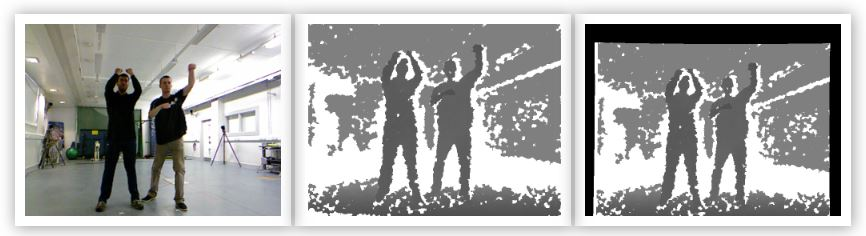
\includegraphics[scale=0.55]{dataset-1.JPG}
	\caption{Left to right : Colour, raw depth and depth transformed to colour co-ordinates}
	\label{fig:Dataset-1}
	\end{figure}

	\begin{figure}[htbp]
	\centering
	\begin{minipage}[t]{0.48\textwidth}
	\centering
	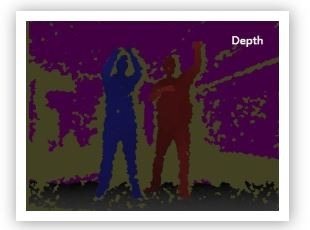
\includegraphics[width=6cm]{dataset-2.JPG}
	\caption{Segmented player}
	\label{fig:Dataset-2}
	\end{minipage}
	\begin{minipage}[t]{0.48\textwidth}
	\centering
	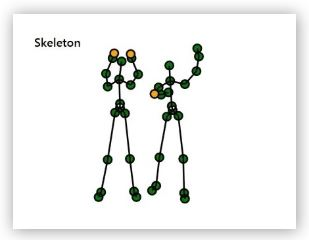
\includegraphics[width=6cm]{dataset-3.JPG}
	\caption{Skeleton}
	\label{fig:Dataset-3}
	\end{minipage}
	\end{figure}

	The summary of the dataset is presented in Table 1.\cite{1} In this paper, we are focusing on using the colour data, which is the original frame, as our research data.

	\begin{table}[!hbp]
	\begin{tabular}{|c|c|c|c|c|c|}
	\hline
	Dataset	& Classes & Subjects & Data Sources & Instruction Modality & Scenario\\
	\hline
	G3Di & 4 & 12 & Colour+Depth + Skeleton & Gamesourced	& Actions + Interactions\\
	\hline
	\end{tabular}
	\caption{Experimental Result}
	\end{table}


\section{Proposed Method}

	The overview of our proposed method has 4 general steps including 1) Create feature histogram; 2) Preprocessing data; 3) Feature Extraction; and 4) Classification. Next, each step is explained in detail. The main purpose is to classify different human actions in video games.

	\subsection{Create Feature Histogram}
		Prepare comparable data is the first step of this system which provides informative data for the next steps. In this paper, for computing the optical flow histogram information of the video, several preprocessing steps are needed. The raw data of the dataset is the png image for every frame of the video. The length of the video is between 300 frames to 3000 frames. To use the raw data, we need to rename the image first, so we can process the image in order. Rename script (ren.bat) written by ourselves has been used. This rename script can rename multiple file name in order at once with the same title provided followed by order number.\\
		After renaming the image name, keyframes need to be select from each type of games. The keyframe video needs to have the same length, so it can be compared with video input later and get a reasonable result. The keyframe video does not need to be an entire action, it should be the part of the action which is special in this action. During the classification, the program can classify the motion by those keyframe video.\\
		The next step is to generate the optical flow vector image between each two frames of keyframe video. Horn-Schunck optical flow method needs to be used in this process. The Horn-Schunck optical flow method is a method can select similar feature pixel in two different images and gives the movement vector for each pixel(more details about Horn-Schunck optical flow method is in 3.3 Feature Extraction). Example of optical flow vector image shown as Fig.\ref{fig:of-1} and Fig.\ref{fig:of-2}. Generate the optical flow vector image for every two frames for keyframe video, so the number of optical flow vector image will be the length by the frame of the keyframe video minus 1. In this study, the keyframe videos have 70 frames and there are 69 optical flow vector images for each keyframe video.

		\begin{figure}[htbp]
		\centering
		\begin{minipage}[t]{0.49\textwidth}
		\centering
		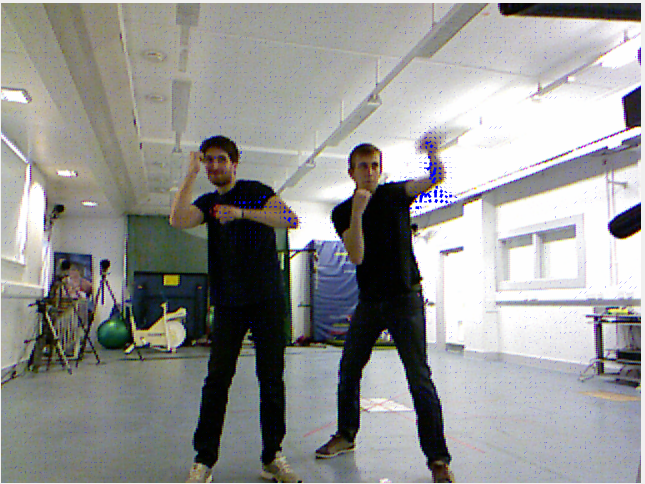
\includegraphics[width=6cm]{opticalflowresult1.png}
		\caption{Optical Flow Result Example}
		\label{fig:of-1}
		\end{minipage}
		\begin{minipage}[t]{0.49\textwidth}
		\centering
		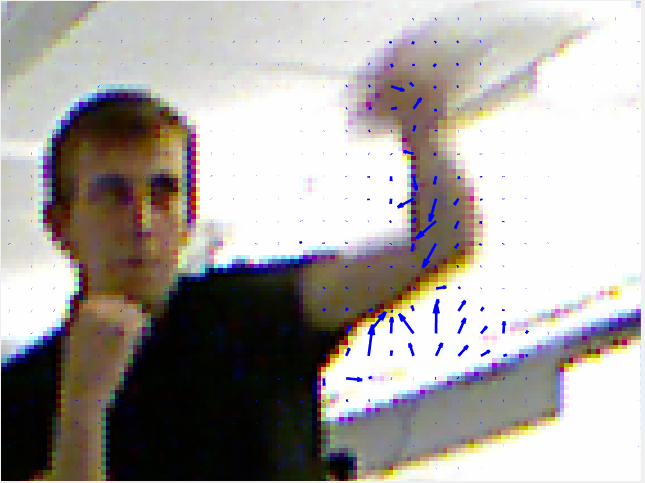
\includegraphics[width=6cm]{opticalflowresult2.png}
		\caption{Example details}
		\label{fig:of-2}
		\end{minipage}
		\end{figure}

		For each optical flow vector image, a threshold is needed to be applied to get rid of the small movement of pixels. The threshold leaves long-distance movement to show the feature for each type of motion. In this study, one of the game types is boxing, it has much short distance movement, so the threshold is 0.05. In other cases the threshold can be different. Then the program will generate two different histograms for each optical flow vector image after a threshold has been applied. The histogram is a count up of different size of movement in each vertical direction and horizontal direction. In this study, the longest distance of movement is 387 pixels, but to make sure every movement will be counted up, we generate the histogram from -500 pixel distance to 500 pixel distance (0 included). Because of the 0 distance movement is meaningless and it affected the result most at the same time, the 0 distance movement needed to be removed from the histogram. The histogram should count up from -500 pixel distance to 500 pixel distance(0 is not included). And this is the feature histogram for comparison. There are 69 feature histograms for each different action. To comparing all the feature histograms at once, the program will glue the histograms up, make them one followed by another in order. The length of the final feature histogram should be\\
		number of frames(|min movement distance| + |max movement distance|) \\
		In this study, the length of final feature histogram is 69 frames $\times$ (|-500|+|500|)=69000. Some examples are shown in Fig.\ref{fig:he-1} - Fig.\ref{fig:he-8} (The left one: X is the length of the histogram Y is the frequency of different movement distance on horizontal direction; The right one: X is the length of the histogram Y is the frequency of different movement distance on vertical direction). And there are four different types of action, so there are four different feature histograms with the same length.


		\begin{figure}[htbp]
		\centering
		\begin{minipage}[t]{0.49\textwidth}
		\centering
		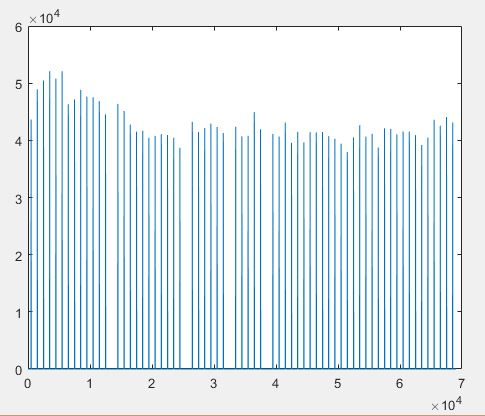
\includegraphics[width=6cm]{footballBoxing-1.JPG}
		\caption{Histogram Example Football vs Boxing-1}
		\label{fig:he-1}
		\end{minipage}
		\begin{minipage}[t]{0.49\textwidth}
		\centering
		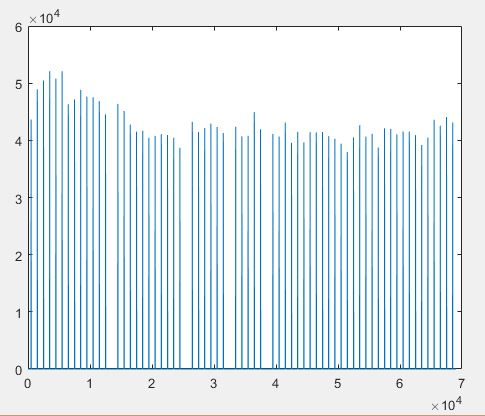
\includegraphics[width=6cm]{footballBoxing-1.JPG}
		\caption{Histogram Example Football vs Boxing-2}
		\label{fig:he-2}
		\end{minipage}
		\end{figure}

		\begin{figure}[htbp]
		\centering
		\begin{minipage}[t]{0.49\textwidth}
		\centering
		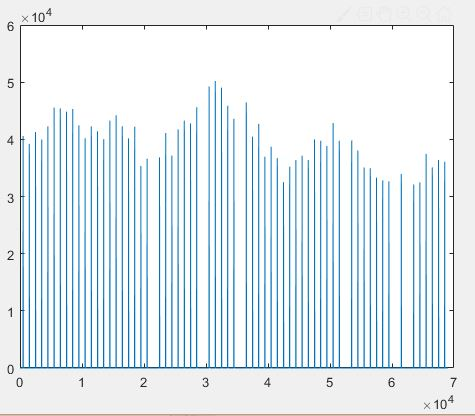
\includegraphics[width=6cm]{footballFootball-1.JPG}
		\caption{Histogram Example Football vs Football-1}
		\label{fig:he-3}
		\end{minipage}
		\begin{minipage}[t]{0.49\textwidth}
		\centering
		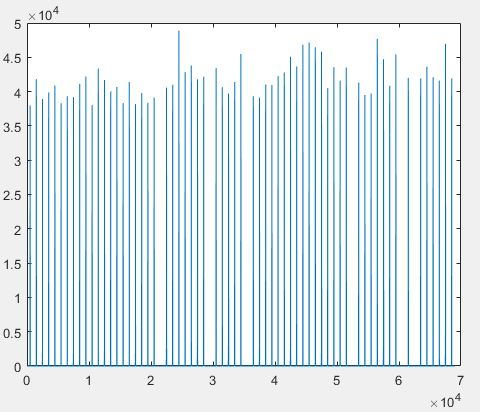
\includegraphics[width=6cm]{footballFootball-2.JPG}
		\caption{Histogram Example Football vs Football-2}
		\label{fig:he-4}
		\end{minipage}
		\end{figure}

		\begin{figure}[htbp]
		\centering
		\begin{minipage}[t]{0.49\textwidth}
		\centering
		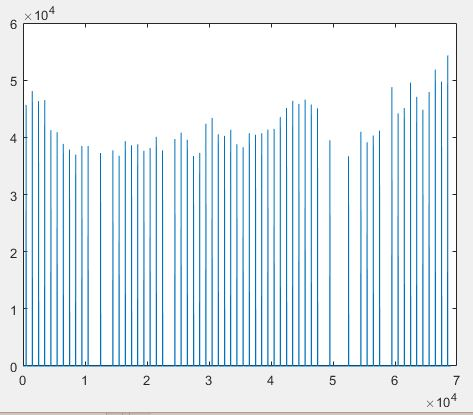
\includegraphics[width=6cm]{footballTabletennis-1.JPG}
		\caption{Histogram Example Football vs Tabletennis-1}
		\label{fig:he-5}
		\end{minipage}
		\begin{minipage}[t]{0.49\textwidth}
		\centering
		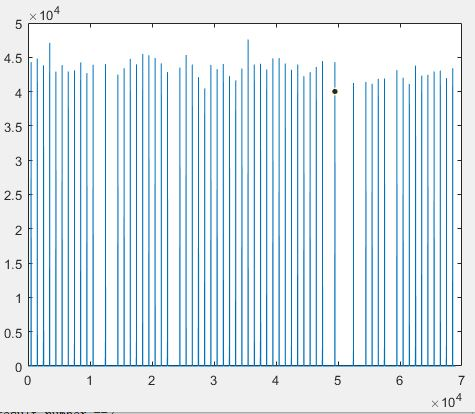
\includegraphics[width=6cm]{footballTabletennis-2.JPG}
		\caption{Histogram Example Football vs Tabletennis-2}
		\label{fig:he-6}
		\end{minipage}
		\end{figure}

		\begin{figure}[htbp]
		\centering
		\begin{minipage}[t]{0.49\textwidth}
		\centering
		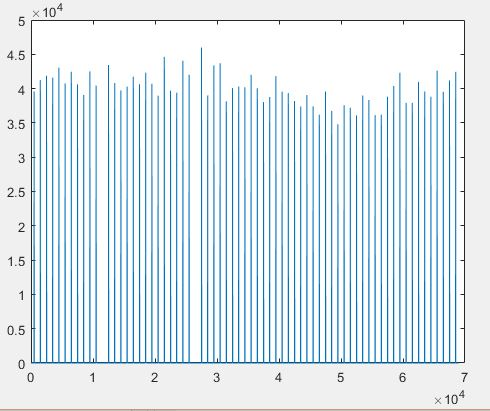
\includegraphics[width=6cm]{footballVolleyball-1.JPG}
		\caption{Histogram Example Football vs Volleyball-1}
		\label{fig:he-7}
		\end{minipage}
		\begin{minipage}[t]{0.49\textwidth}
		\centering
		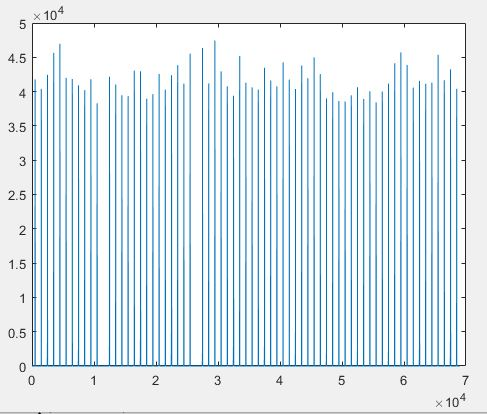
\includegraphics[width=6cm]{footballVolleyball-2.JPG}
		\caption{Histogram Example Football vs Volleyball-2}
		\label{fig:he-8}
		\end{minipage}
		\end{figure}

\vbox{}
\vbox{}
\vbox{}
\vbox{}
\vbox{}
\vbox{}
\vbox{}
\vbox{}
\vbox{}
\vbox{}
\vbox{}
\vbox{}
\vbox{}
\vbox{}
\vbox{}
	\subsection{Preprocessing Data}

		After feature histograms have been created, the next step is comparing the input video with the feature histograms to start to recognize the human action in the video game. Before the comparison, the program needs to preprocess the input video. Not likely creating feature histogram, we don’t select keyframes from the input video. The program needs to generate the optical flow vector images for the entire input video by using the Horn-Schunck optical flow method(details see 3.3 Feature Extraction). After using the Horn-Schunck optical flow method to generate the optical flow vector image, we use a threshold to get rid of 0 distance movement and combined them as a long histogram. The length of the final histogram  should be\\
		number of frames(|min movement distance| + |max movement distance|) \\
		Because of the number of the frames are different in different videos, the length of the histogram will be different as well.\\
		Image offset, such as camera shaking sometimes will cause a very bad result. To get rid of the small image offset, there are two more thresholds will be applied to the input video histogram. One is a vertical threshold, which removes movement distance frequency higher than 120000 in a vertical direction.  The other one is a horizontal threshold, which removes movement distance frequency higher than 70000 in a horizontal direction. Because of the image offset will cause all of the pixels to move to the same direction in a short distance, the threshold of high frequency on both vertical and horizontal direction can efficiently solve this problem. The example of the final input video histogram shown in Fig.\ref{fig:his-11} (X is the length of the histogram Y is the frequency of different movement distance on horizontal direction) and Fig.\ref{fig:his-12} (X is the length of the histogram Y is the frequency of different movement distance on vertical direction).

		\begin{figure}[htbp]
		\centering
		\begin{minipage}[t]{0.49\textwidth}
		\centering
		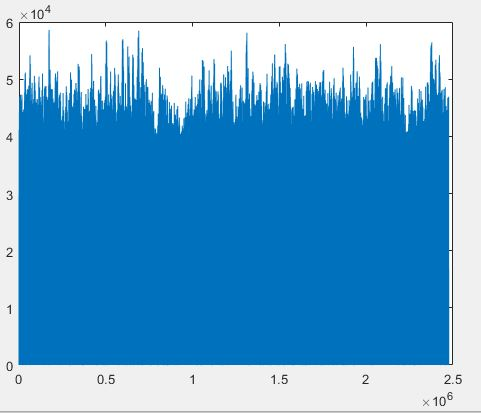
\includegraphics[width=6cm]{his-3_x.JPG}
		\caption{Input video histogram-1)}
		\label{fig:his-11}
		\end{minipage}
		\begin{minipage}[t]{0.49\textwidth}
		\centering
		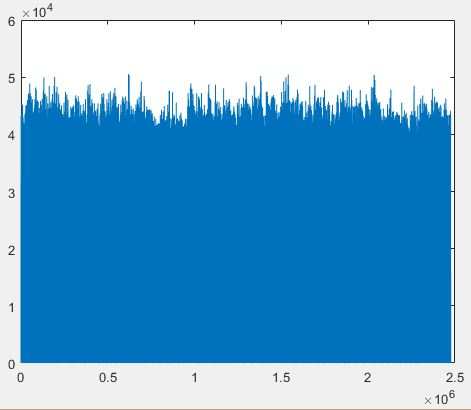
\includegraphics[width=6cm]{his-3_y.JPG}
		\caption{Input video histogram-2)}
		\label{fig:his-12}
		\end{minipage}
		\end{figure}

	\subsection{Feature Extraction}

		In 1981, Horn and Schunck put forward an additional constraint condition according to the continuous and smooth characteristics of the optical flow field of the same moving object and converted the overall smooth constraint of the optical flow field into a variational problem, this method called Horn-Schunck optical flow method.\cite{3}\\

		\subsubsection{Algorithm Assumptions:}
			\paragraph{}
			Horn-Schunck optical flow algorithm uses a global method to estimate the dense optical flow field of an image (that is, to calculate the optical flow for each pixel in the image). The algorithm is based on two assumptions\cite{4}\\

			\begin{enumerate}
			\item The grayscale is invariant\\
			Even if the object moves, the grayscale of the same point on the object is constant in the image. (this assumption can be satisfied under stable illumination, but it is not true for images with high light reflection.)\\
			\item The optical flow field is smooth\\
			Pixels belonging to the same object in the scene should form a smooth optical flow field vector, and the optical flow will only mutate at the boundary of the object which is only a small part of the image. In general, the optical flow field of the image should be smooth. \\
			\end{enumerate}
\vbox{}

		\subsubsection{Algorithm Flowchart: }
			%\paragraph{}
			We improved the HS algorithm method according to Enric Meinhardt-Llopis, the classic HS method is shown in Algorithm 1.\cite{5} Our HS algorithm method is shown in Algorithm 2.\\

				\begin{algorithm}[h]
				\caption{Classic HS method Algorithm}
				\begin{algorithmic}[1]

				\REQUIRE I, $\alpha$, $\varepsilon$ \\ 
				\ENSURE h = (u,v)\\
				\STATE Compute $I_x$, $I_y$, $I_t$
				\STATE $u \Leftarrow 0$
				\STATE $v \Leftarrow 0$
				\STATE $n \Leftarrow 0$

				\WHILE{$n < N_maxiter$ and $stopping\_criterion > \varepsilon $} 
				\STATE Compute $\overline{u}$, $\overline{v}$
				\STATE $u \Leftarrow \overline{u} - I_x \frac{I_x\overline{u} + I_y\overline{v} + I_t}{\alpha^2 + I_x^2 + I_y^2}$ 
				\STATE $v \Leftarrow \overline{v} - I_y \frac{I_x\overline{u} + I_y\overline{v} + I_t}{\alpha^2 + I_x^2 + I_y^2}$
				\STATE $Compute stopping\_criterion$ 
				\STATE $n \Leftarrow n + 1$ 
				\ENDWHILE

				\label{code:recentEnd}
				\end{algorithmic}
				\end{algorithm}

				\begin{algorithm}[h]
				\caption{HS method Algorithm Flowchart}
				\begin{algorithmic}[1]

				\REQUIRE frame1, frame2\\ 
				Build image pyramid;\\
				Initialize flow = 0;\\
				\FOR{each $i \in [1,numPyramidLevel]$}
				\STATE Initialize flow from previous level;\
				\STATE Build gradient matrix and Laplacian matrix;\
				\STATE{
				\FOR{each $j \in [1,maxWarpingNum]$} 
				\STATE{Warp image using flow vector;}
				\STATE{Compute image gradient Ix, Iy, and Iz;}
				\STATE{Build linear system to solve HS flow;}
				\STATE{Solve linear system to compute the flow;}
				\STATE{Use median filter to smooth the flow map;}
				\ENDFOR}
				\ENDFOR
				\ENSURE flow;\\
				\label{code:recentEnd}
				\end{algorithmic}
				\end{algorithm}

\vbox{}
\vbox{}
\vbox{}
\vbox{}


		\subsubsection{Main Formula}
			\paragraph{}
			The algorithm constructs an energy function, which transforms the problem of finding the optical flow field into finding the minimum value of the energy function.\cite{19}\\
			1 $$E = \int \int [(I_xu+I_yv+I_t)^2 + \alpha^2(|\nabla u|^2 + |\nabla v|^2)]dxdy$$\\
			2 $$\frac{\partial L}{\partial u} - \frac{\partial}{\partial x}\frac{\partial L}{\partial u_x} = \frac{\partial}{\partial y}\frac{\partial L}{\partial u_y}= 0$$\\
			3 $$\frac{\partial L}{\partial v} - \frac{\partial}{\partial x}\frac{\partial L}{\partial v_x} = \frac{\partial}{\partial y}\frac{\partial L}{\partial v_y}= 0$$\\
			4 $$I_x(I_xu + I_yv + I_t)-\alpha^2\Delta u= 0$$\\
			  $$I_y(I_xu + I_yv + I_t)-\alpha^2\Delta v= 0$$\\
			5 $$\Delta = \frac{\partial^2}{\partial x^2} + \frac{\partial^2}{\partial y^2}$$\\
			6 $$u^{k+1} = u^{-k} - \frac{I_x(I_xu^{-k} + I_t)}{\alpha^2 + I_x^2 + I_y^2}$$
			  $$v^{k+1} = v^{-k} - \frac{I_y(I_xu^{-k} + I_t)}{\alpha^2 + I_x^2 + I_y^2}$$\\

	\subsection{Classification}
		In this part, the aim is to find out if the feature histogram is part of the input video histogram or similar to the part of the input video histogram. So the input video can be classified as the most similar feature histogram type of action.\\
		At first, because of different actions have a different amount of movement distance, it’s easy to classify some of them by analyzing their histogram data. In this study, boxing has the smallest amount of movement and because of the volleyball need to jump, so it has the largest amount of movement. For table tennis and football, they have a similar amount of movement. The total amount of movement can be calculated by the function,\\
		$$M = \sum_{x} h + \sum_{y} h$$   Where h represents the histogram of the input video.\\
		In this study, if M is smaller than 200000000, then the input video action can be classified as boxing. And if M is greater than 770000000, then the input video can be classified as volleyball.\\
		For the actions have a similar amount of movement, we have to use histogram subtraction to calculate the distance between the input video histogram and the feature histogram. In this study, the feature histogram has only 69 frames, but the input video can be any frames. The histogram of any 69 continuous frames in the input video can be similar to the feature histogram.
		By switch one frame at once, the input video histogram and the feature histogram need to compare m-n+1 times, which m is the input video’s frames and n is the feature video frames.\\
		For each comparison the difference between two histogram is\\
		$$d = \sum_{x} (\sqrt{h_{1}} - \sqrt{h_{2}}) + \sum_{y} (\sqrt{h_{1}} - \sqrt{h_{2}})$$ Where h1 is the first histogram and h2 is the second histogram.\\
		Then in all of comparison, the smallest distance represents the most similar result between the feature histogram and the input video histogram.\\
		$$d = min(\sum_{x} (\sqrt{h_{1}} - \sqrt{h_{2}}) + \sum_{y} (\sqrt{h_{1}} - \sqrt{h_{2}}))$$\\
		After comparing with different type of feature histograms, the action type of smallest result represents the class of the input video.

\section{Results and Discussion}

	In this study, the dataset G3Di has four categories and six videos for each category. Each video has two players showing the action at the same time. Four categories are boxing, football, table tennis, and volleyball. After using our human action recognize algorithm, the overall accuracy is  75.0\%, more details shown table blow.\\

	From Table 2 we can see, the accuracy of boxing type action recognition is 100.00\% and the accuracy of volleyball type action recognition is 83.33\%. The accuracy is higher than 80\% shows the data analyzing is successful. \\
	The other two types of actions have lower recognition accuracy because in the video there are two players showing the action at the same time. The overlapping of actions makes the histogram subtraction harder. Sometimes the algorithm cannot find a similar part of the histogram. If the dataset can be separated by using Histogram of Oriented Gradients(HOG) \cite{6} using Support Vector Machine(SVM) method\cite{7} as the classifier to recognize one person each time, the accuracy can be much higher.\\

	\begin{table}[!hbp]\small
	\begin{tabular}{|c|c|c|c|c|}
	\hline
	Category & Data set & Recognition Result & Accuracy & Total accuracy\\
	\hline
	\multirow{6}{*}{Boxing} & Boxing\_{}p5\&p6 & Boxing & \multirow{6}*{100\%}  & \multirow{24}*{75.00\%}\\
	\cline{2-3}
	& Boxing\_{}p7\&p8 & Boxing &  & \\
	\cline{2-3}
	& Boxing\_{}p9\&p10 & Boxing &  & \\
	\cline{2-3}
	& Boxing\_{}p11\&p12 & Boxing &  & \\
	\cline{2-3}
	& Boxing\_{}p13\&p14 & Boxing &  & \\
	\cline{2-3}
	& Boxing\_{}p15\&p16 & Boxing &  & \\
	\cline{1-4}
	\multirow{6}{*}{FootBall} & FootBall\_{}p5\&p6 & FootBall & \multirow{6}*{50.00\%}  &  \\
	\cline{2-3}
	& FootBall\_{}p7\&p8 & TableTennis &  & \\
	\cline{2-3}
	& FootBall\_{}p9\&p10 & FootBall &  & \\
	\cline{2-3}
	& FootBall\_{}p11\&p12 & FootBall &  & \\
	\cline{2-3}
	& FootBall\_{}p13\&p14 & Volleyball &  & \\
	\cline{2-3}
	& FootBall\_{}p15\&p16 & TableTennis &  & \\
	\cline{1-4}
	\multirow{6}{*}{TableTennis} & TableTennis\_{}p5\&p6 & TableTennis & \multirow{6}*{66.67\%}  &  \\
	\cline{2-3}
	& TableTennis\_{}p7\&p8 & TableTennis &  & \\
	\cline{2-3}
	& TableTennis\_{}p9\&p10 & FootBall &  & \\
	\cline{2-3}
	& TableTennis\_{}p11\&p12 & TableTennis &  & \\
	\cline{2-3}
	& TableTennis\_{}p13\&p14 & TableTennis &  & \\
	\cline{2-3}
	& TableTennis\_{}p15\&p16 & TableTennis &  & \\
	\cline{1-4}
	\multirow{6}{*}{Volleyball} & Volleyball\_{}p5\&p6 & Volleyball & \multirow{6}*{83.33\%}  &  \\
	\cline{2-3}
	& Volleyball\_{}p7\&p8 & Volleyball &  & \\
	\cline{2-3}
	& Volleyball\_{}p9\&p10 & Volleyball &  & \\
	\cline{2-3}
	& Volleyball\_{}p11\&p12 & FootBall &  & \\
	\cline{2-3}
	& Volleyball\_{}p13\&p14 & Volleyball &  & \\
	\cline{2-3}
	& Volleyball\_{}p15\&p16 & Volleyball &  & \\
	\hline
	\end{tabular}
	\caption{Experimental Result}
	\end{table}

	

	\begin{table}[!hbp]
	\begin{tabular}{|p{1.5cm}|p{2cm}|p{3.5cm}|p{2.5cm}|p{1cm}|p{1.5cm}|}
	\hline
	Method & Name & Description & Scholarly Article & Publish Year & Author(s)\\
	\hline

	AdaBoost & - & AdaBoost was trained on the source dataset and the parameters: the number of training frames around each peak pose the sliding smoothing window size were optimised on the training part of the target dataset and the method was evaluated on to the target testing data. & Human Action Recognition Based on AdaBoost Algorithm for Feature Extraction & 2014 Sept. & Xiaofei Ji, Lu Zhou, Yibo Li\\
	\hline

	CSTM & Clustered Spatio-Temporal Manifolds & CSTM trained on the source dataset and the parameters: the template size and the peak pose detector were optimised on the training part of the target dataset and the method was evaluated on to the target testing data. & Clustered Spatio-temporal Manifolds for Online Action Recognition & 2014 Aug. & Victoria Bloom, Dimitrios Makris, Vasileios Argyriou\\
	\hline

	PSM & Peak Segment Matching & An extension of CSTM which instead of a binary decision for matching a peak key pose introduces a threshold to detect actions with extended duration. & - & - & -\\
	\hline

	BPM & Body Part Matching & An extension of PSM which instead of using the standard DTW(Dynamic Time Warping) in the matching process, uses a selective DTW based on the most discriminative body parts to detect compound actions. & - & - & -\\
	\hline

	TLM & Transfer Learning Matching & An extension of PSM which instead of training and testing on the same dataset. Learns the action templates on a simpler dataset, and performs model adaption on a more complex dataset. & Transfer Learning for Activity Recognition: A Survey & 2013 Sept. & Diane Cook, Kyle D. Feuz, Narayanan C. Krishnan\\
	\hline

	HTL & Hierarchical Transfer Learning framework & Transfer learning is applied to Peak Segment Matching, allowing knowledge to be transferred from simple actions in a source dataset to compound actions in a target dataset by adapting the body part models and peak key poses. & Hierarchical Transfer Learning for Online Recognition of Compound Actions & 2015 Dec. & Victoria Bloom, Vasileios Argyriou, Dimitrios Makris\\
	\hline

	\end{tabular}
	\caption{Exist Methods}
	\end{table}

	\begin{figure}[htbp]
	\centering
	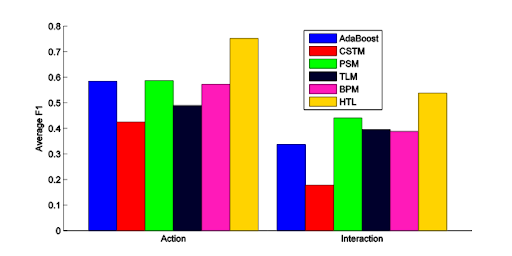
\includegraphics[scale=0.8]{previous-1.png}
	\caption{ Performance comparison of the different approaches. The proposed method (HTL) outperforms the others for both action and interaction detection. }
	\label{fig:p-1}
	\end{figure}

	\begin{figure}[htbp]
	\centering
	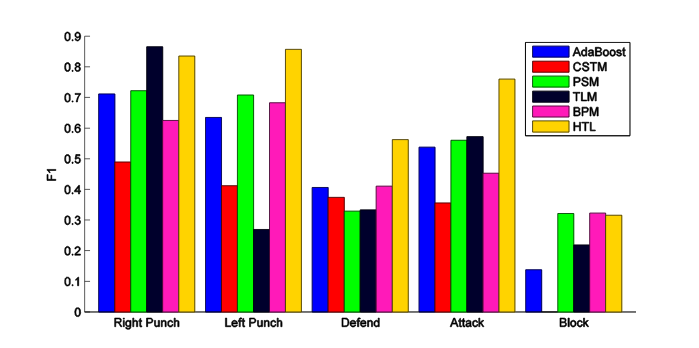
\includegraphics[scale=0.48]{previous-2.png}
	\caption{ Action recognition results for each category of the G3Di (Fighting) dataset using different algorithms
	 }
	\label{fig:p-2}
	\end{figure}

	Result from other methods are shown in Fig.\ref{fig:p-1} and Fig.\ref{fig:p-2}. According to Fig.\ref{fig:p-2}, so far, by using G3Di as dataset, there is no algorithm to achieve the accuracy of more than 90\%. The highest one is using TLM and its accuracy is between 80\% to 90\%.Our method has 75.00\% accuracy which is higher than the average, but it is still not the best. 

	\vbox{}
	\vbox{}
	\vbox{}
	\vbox{}
	\vbox{}
	\vbox{}
	\vbox{}
	\vbox{}

\section{Conclusion}

	In this paper, we presented the optical flow and histogram analysis method for human action recognition. We overcome the problem of distinguishing multiplayer simultaneous movement and the result demonstrates that our method is accurate for action recognition. Although our approach has achieved considerable accuracy, there are still many factors to be improved. For example, if the two people in the video are analyzed separately, the error may be reduced; if the interference factor in the background can be minimized, the accuracy may be improved, and so on. We will continue to explore these potential extensions to improve the efficiency and accuracy of our approach.


\begin{thebibliography}{4}

\bibitem{1} V. Bloom, V. Argyriou and D. Makris, "Hierarchical transfer learning for online recognition of compound actions", Computer Vision and Image Understanding, vol. 144, pp. 62-72, 2016. http://dipersec.king.ac.uk/G3D/G3Di.html.

\bibitem{2} S., H. W. and Gibson, James J. (1951). The Perception of the Visual World. \_Journal of Philosophy\_ 48 (25):788.

\bibitem{3} Pinto, Andry \& Moreira, A \& Costa, Paulo \& Correia, Miguel. (2013). Revisiting Lucas-Kanade and Horn-Schunck. Journal of Computer Engineering and Informatics. 1. 23-29. 10.5963/JCEI0102001. 

\bibitem{4} https://fzheng.me/2015/03/25/optical-flow/

\bibitem{5} Enric Meinhardt-Llopis, Javier Sánchez Pérez, and Daniel Kondermann, Horn-Schunck Optical Flow with a Multi-Scale Strategy, Image Processing On Line, 3 (2013), pp. 151–172. https://doi.org/10.5201/ipol.2013.20



\bibitem{6} Liu, Hong \& Xu, Tao \& Wang, Xiangdong \& Qian, Yueliang. (2013). Related HOG Features for Human Detection Using Cascaded Adaboost and SVM Classifiers. 10.1007/978-3-642-35728-2\_33.

\bibitem{7} Eftakhar, Ashik \& Kooi Tan, Joo \& Kim, Hyoungseop \& Ishikawa, S. (2011). Multiple persons' action recognition by fast human detection. 1639-1644.

\bibitem{8} Z. Jiang, Z. Lin and L. Davis, "Recognizing Human Actions by Learning and Matching Shape-Motion Prototype Trees," in IEEE Transactions on Pattern Analysis and Machine Intelligence, vol. 34, no. 3, pp. 533-547, March 2012.

\bibitem{9} Zhe Lin, Zhuolin Jiang, and Larry S. Davis, "Recognizing Actions by Shape-Motion Prototype Trees, " IEEE 12th International Conference on Computer Vision (ICCV), pp.444-451, 2009.

\bibitem{10} Bloom, Victoria (2015) Multiple Action Recognition for Video Games (MARViG). (PhD thesis), Kingston University. 

\bibitem{11} F. Porikli, “Integral Histogram: A Fast Way to Extract Histograms in Cartesian Spaces”, Proc. of International Conference on Computer Vision and Pattern Recognition (CVPR), Vol. 1, pp. 829-836, 2005.

\bibitem{12} Yansong Tang, Zian Wang, Peiyang Li, Jiwen Lu, Ming Yang, Jie Zhou: Mining Semantics-Preserving Attention for Group Activity Recognition. ACM Multimedia 2018: 1283-1291

\bibitem{13} M.Jones, P.Viola. Fast Multi-View Face Detection. Mitsubishi Electric Research Laboratories, Technical Report: MERL-2003-96, July 2003.

\bibitem{14} Vrigkas, Michalis \& Nikou, Christophoros \& Kakadiaris, Ioannis. (2015). A Review of Human Activity Recognition Methods. Frontiers in Robotics and Artificial Intelligence. 2. 10.3389/frobt.2015.00028. 

\bibitem{15} Luis Alvarez, Joachim Weickert, and Javier S ́anchez. Reliable esti  ́ mation of dense optical flow fields with large displacements. International Journal of Computer Vision, 39(1):41–56, 2000. http://dx.doi.org/10.1023/A:1008170101536.

\bibitem{16} Simon Baker, Daniel Scharstein, J. P. Lewis, Stefan Roth, Michael J. Black, and Richard Szeliski. A database and evaluation methodology for optical flow. In International Conference on Computer Vision, pages 1–8, 2007. http://dx.doi.org/10.1109/ICCV.2007.4408903.

\bibitem{17} Satish Balay, Kris Buschelman, William D. Gropp, Dinesh Kaushik, Matthew G. Knepley, Lois Curfman McInnes, Barry F. Smith, and Hong Zhang. PETSc Web page, 2001. http://www.mcs.anl.gov/petsc.

\bibitem{18} Satish Balay, William D. Gropp, Lois Curfman McInnes, and Barry F. Smith. Efficient management of parallelism in object oriented numerical software libraries. In E. Arge, A. M. Bruaset, and H. P. Langtangen, editors, Modern Software Tools in Scientific Computing, pages 163–202. Birkh ̈auser Press, 1997. http://dx.doi.org/10.1007/978-1-4612-1986-6\_8.

\bibitem{19} https://en.wikipedia.org/wiki/Horn\%E2\%80\%93Schunck\_method

\bibitem{20} Nils Papenberg, Andr ́es Bruhn, Thomas Brox, Stephan Didas, and Joachim Weickert. Highly Accurate Optic Flow Computation with Theoretically Justified Warping. Interna-tional Journal of Computer Vision, 67(2):141–158, April 2006. http://dx.doi.org/10.1007/s11263-005-3960-y.

\bibitem{21} M. Lewandowski, D. Makris, J. Nebel, Temporal extension of Laplacian eigenmaps for unsupervised dimensionality reduction of time series, in: Proceedings of International Conference on Pattern Recognition, 2010, pp. 161–164. 

\bibitem{22} T. Kanungo, D.M. Mount, N.S. Netanyahu, A.Y. Wu, C.D. Piatko, A local search approximation algorithm for k-means clustering, in: Proceedings of Special Issue 18th Annual Symposium on Computational Geometry - SoCG2002, 28, 2003, pp. 89–112. 
\bibitem{23} P. Senin, Dynamic Time Warping Algorithm Review, University of Hawaii, USA, 2008. 

\bibitem{24} I. Kviatkovsky, E. Rivlin, I. Shimshoni, Online action recognition using covariance of shape and motion, Comput. Vis. Image Underst. 129 (Dec. 2014) 15–26.

\bibitem{25} S.K. Card, G.G. Robertson, J.D. Mackinlay, The information visualizer: an information workspace, in: Proceedings of ACM CHI, 1991, pp. 181–188. 

\bibitem{26} J. Shotton, A. Fitzgibbon, M. Cook, T. Sharp, M. Finocchio, R. Moore, A. Kipman, A. Blake, Real-time human pose recognition in parts from a single depth image, in: Proceedings of IEEE CVPR, 2011.


\end{thebibliography}

\end{document}
